\documentclass{article}
\usepackage[margin=0.8cm]{geometry}
\usepackage{tikz}
\usetikzlibrary{arrows.meta,positioning,shapes.geometric,calc,fit,backgrounds}

\pagestyle{empty}

% Target column width for IEEE two-column layout (~8.5 cm)
\newcommand{\colw}{8.5cm}

\begin{document}
	
	%% ════════════════════════════════════════════════════════════════════════
	%%  FIGURE 1 — Offline Model Development Pipeline (PC side)
	%% ════════════════════════════════════════════════════════════════════════
	\noindent\resizebox{\colw}{!}{%
		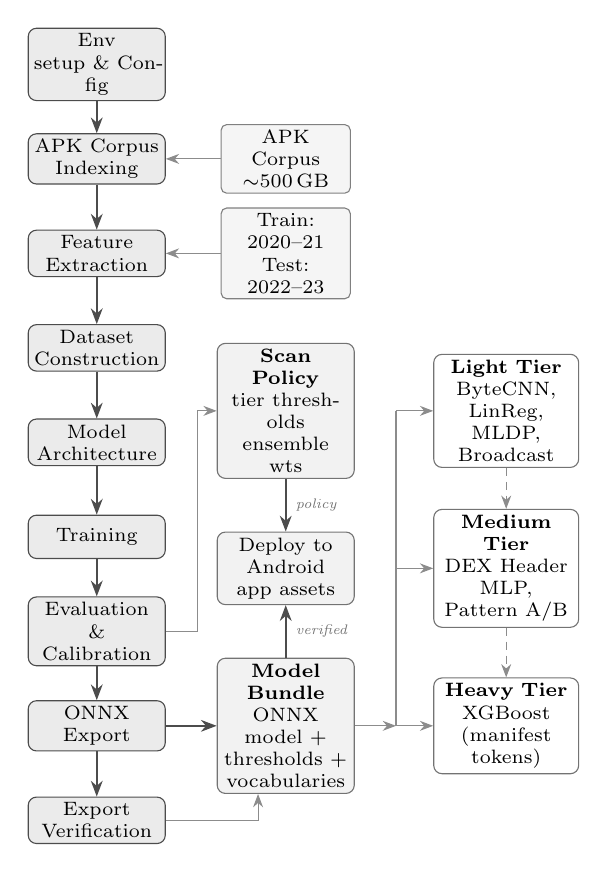
\begin{tikzpicture}[
			font=\scriptsize,
			>=Stealth,
			phase/.style={
				rectangle, rounded corners=3pt,
				draw=black!70, fill=black!8,
				text width=1.6cm, align=center,
				minimum height=0.55cm, inner sep=2pt
			},
			tierbox/.style={
				rectangle, rounded corners=3pt,
				draw=black!55, fill=white,
				text width=1.7cm, align=center,
				minimum height=0.55cm, inner sep=2pt
			},
			side/.style={
				rectangle, rounded corners=2pt,
				draw=black!50, fill=black!4,
				text width=1.5cm, 
				align=center,
				minimum height=0.5cm, inner sep=2pt
			},
			mid/.style={
				rectangle, rounded corners=3pt,
				draw=black!55, fill=black!5,
				text width=1.6cm, align=center,
				minimum height=0.55cm, inner sep=2pt
			},
			arr/.style={->, semithick, black!70},
			sarr/.style={->, thin, black!45},
			lbl/.style={font=\tiny\itshape, black!55}
			]
			
			%% ── Main spine (left column, x=0) ───────────────────────────────────
			\node[phase] (setup) at (0,  0.0) {Env setup~\&~Config};
			\node[phase] (index) at (0, -1.2) {APK Corpus\\Indexing};
			\node[phase] (feat)  at (0, -2.4) {Feature\\Extraction};
			\node[phase] (load)  at (0, -3.6) {Dataset\\Construction};
			\node[phase] (arch)  at (0, -4.8) {Model\\Architecture};
			\node[phase] (train) at (0, -6.0) {Training};
			\node[phase] (eval)  at (0, -7.2) {Evaluation \&\\Calibration};
			\node[phase] (onnx)  at (0, -8.4) {ONNX\\Export};
			\node[phase] (parity)at (0, -9.6) {Export\\Verification};
			
			\foreach \a/\b in {setup/index, index/feat, feat/load, load/arch,
				arch/train, train/eval, eval/onnx, onnx/parity}
			\draw[arr] (\a) -- (\b);
			
			%% ── Middle column / Inputs (aligned at x=2.4) ───────────────────────
			\node[side] (corpus) at (2.4, -1.2) {APK Corpus\\$\sim$500\,GB};
			\node[side] (split)  at (2.4, -2.4) {Train: 2020--21\\Test: 2022--23};
			
			\node[mid] (policy) at (2.4, -4.4) {
				\textbf{Scan Policy}\\
				tier thresholds\\
				ensemble wts
			};
			
			\node[mid] (phone) at (2.4, -6.4) {
				Deploy to\\Android\\app assets
			};
			
			\node[mid, minimum height=0.65cm] (bundle) at (2.4, -8.4) {
				\textbf{Model Bundle}\\
				ONNX model +\\
				thresholds +\\
				vocabularies
			};
			
			%% Inputs → Main Spine
			\draw[sarr] (corpus.west) -- (index.east);
			\draw[sarr] (split.west)  -- (feat.east);
			
			%% eval → policy (routes safely up and over)
			\draw[sarr] (eval.east) -- ++(0.4,0) |- (policy.west);
			
			%% onnx → bundle
			\draw[arr] (onnx.east) -- (bundle.west);
			
			%% parity → bundle
			\draw[sarr] (parity.east) -| ([xshift=-10pt]bundle.south);
			
			%% ── Central App Deployment Routing ──────────────────────────────────
			%% Policy down to Phone
			\draw[arr] (policy.south) -- node[right, lbl] {policy} (phone.north);
			
			%% Bundle up to Phone
			\draw[arr] (bundle.north) -- node[right, lbl] {verified} (phone.south);
			
			%% ── Right column (tightened to x=5.2) ───────────────────────────────
			\node[tierbox] (tlight) at (5.2, -4.4) {
				\textbf{Light Tier}\\
				ByteCNN, LinReg,\\
				MLDP, Broadcast
			};
			
			\node[tierbox] (tmed) at (5.2, -6.4) {
				\textbf{Medium Tier}\\
				DEX Header MLP,\\
				Pattern A/B
			};
			
			\node[tierbox] (theavy) at (5.2, -8.4) {
				\textbf{Heavy Tier}\\
				XGBoost\\(manifest tokens)
			};
			
			%% ── Unified Shared Bus Routing ──────────────────────────────────────
			%% The bus runs vertically at x=3.8 from y=-4.4 down to y=-8.4
			\draw[draw=black!45, thin] (3.8, -4.4) -- (3.8, -8.4);
			
			%% Mid lane (Bundle only) connecting to the bus
			\draw[sarr] (bundle.east) -- (3.8, -8.4);
			
			%% Bus connecting to the Tiers (Right lane)
			\draw[sarr] (3.8, -4.4) -- (tlight.west);
			\draw[sarr] (3.8, -6.4) -- (tmed.west);
			\draw[sarr] (3.8, -8.4) -- (theavy.west);
			
			%% Cascading dashed arrows between tiers
			\draw[sarr, densely dashed] (tlight.south) -- (tmed.north);
			\draw[sarr, densely dashed] (tmed.south) -- (theavy.north);
			
		\end{tikzpicture}%
	}
	
	\vspace{4pt}
	\noindent\scriptsize\textbf{Fig.\,1.} Offline model-development pipeline.
	
	\newpage
	
	%% ════════════════════════════════════════════════════════════════════════
	%%  FIGURE 2 — On-Device VigiDroid Application Flow
	%% ════════════════════════════════════════════════════════════════════════
	\noindent\resizebox{\colw}{!}{%
		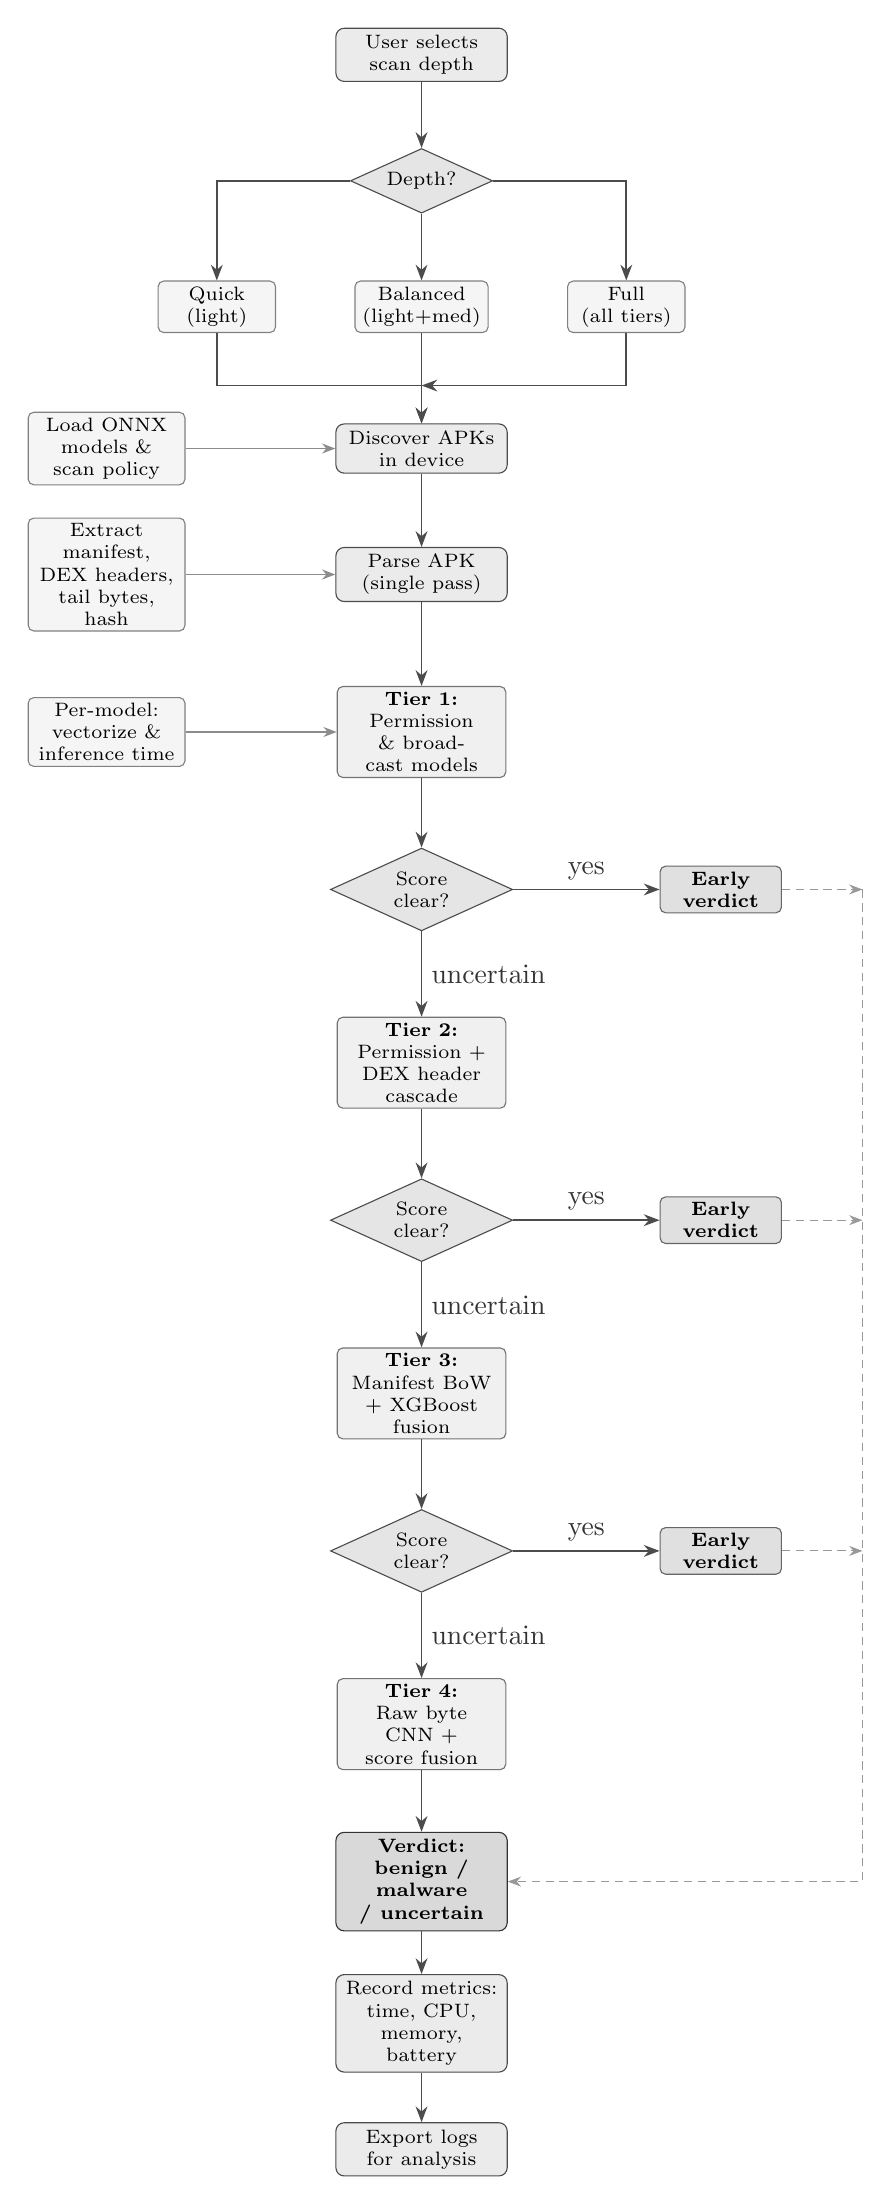
\begin{tikzpicture}[
			font=\scriptsize,
			>=Stealth,
			main/.style={
				rectangle, rounded corners=3pt,
				draw=black!70, fill=black!8,
				text width=2.0cm, align=center,
				minimum height=0.58cm, inner sep=2.5pt
			},
			decision/.style={
				diamond, aspect=2.2,
				draw=black!70, fill=black!10,
				text width=1.1cm, align=center,
				inner sep=1pt
			},
			verdict/.style={
				rectangle, rounded corners=3pt,
				draw=black!80, fill=black!15,
				text width=2.0cm, align=center,
				minimum height=0.55cm, inner sep=2.5pt,
				font=\scriptsize\bfseries
			},
			side/.style={
				rectangle, rounded corners=2pt,
				draw=black!50, fill=black!4,
				text width=1.85cm, align=center,
				minimum height=0.5cm, inner sep=2pt
			},
			tiernode/.style={
				rectangle, rounded corners=2pt,
				draw=black!55, fill=black!6,
				text width=2.0cm, align=center,
				minimum height=0.5cm, inner sep=2pt
			},
			exitnode/.style={
				rectangle, rounded corners=2pt,
				draw=black!60, fill=black!12,
				text width=1.4cm, align=center,
				minimum height=0.42cm, inner sep=2pt,
				font=\scriptsize\bfseries
			},
			arr/.style={->, semithick, black!70},
			sarr/.style={->, thin, black!45},
			darr/.style={->, densely dashed, thin, black!40},
			lbl/.style={font=\scriptsize, black!60}
			]
			
			%% ── Top: user interaction ────────────────────────────────────────────
			\node[main] (ui) at (0, 0.0) {User selects\\scan depth};
			\node[decision] (depth) at (0, -1.6) {Depth?};
			
			\node[side, text width=1.35cm] (dq) at (-2.6, -3.2) {Quick\\(light)};
			\node[side, text width=1.55cm] (db) at ( 0.0, -3.2) {Balanced\\(light+med)};
			\node[side, text width=1.35cm] (df) at ( 2.6, -3.2) {Full\\(all tiers)};
			
			\draw[arr] (ui) -- (depth);
			\draw[arr] (depth.west) -| (dq.north);
			\draw[arr] (depth.south) -- (db.north);
			\draw[arr] (depth.east) -| (df.north);
			
			%% ── Merge to scan ───────────────────────────────────────────────────
			\node[main] (scan) at (0, -5.0) {Discover APKs\\in device};
			
			\draw[arr] (dq.south) -- (-2.6, -4.2) -- (0, -4.2) -- (scan.north);
			\draw[arr] (df.south) -- ( 2.6, -4.2) -- (0, -4.2);
			\draw[arr] (db.south) -- (scan.north);
			
			%% ── Parse once ──────────────────────────────────────────────────────
			\node[main] (parse) at (0, -6.6) {Parse APK\\(single pass)};
			\draw[arr] (scan) -- (parse);
			
			%% ── Tier 1 ──────────────────────────────────────────────────────────
			\node[tiernode] (t1) at (0, -8.6) {
				\textbf{Tier 1:} Permission\\
				\& broadcast models
			};
			\draw[arr] (parse) -- (t1);
			
			%% ── Left annotations — properly spaced out ──────────────────────────
			\node[side] (rscan) at (-4.0, -5.0) {
				Load ONNX\\
				models \&\\
				scan policy
			};
			\draw[sarr] (rscan.east) -- (scan.west);
			
			\node[side] (fctx) at (-4.0, -6.6) {
				Extract manifest,\\
				DEX headers,\\
				tail bytes, hash
			};
			\draw[sarr] (fctx.east) -- (parse.west);
			
			\node[side] (rmetric) at (-4.0, -8.6) {
				Per-model:\\
				vectorize \&\\
				inference time
			};
			\draw[sarr] (rmetric.east) -- (t1.west);
			
			%% ── Tier Decisions — Deep vertical gaps for arrows ──────────────────
			\node[decision] (d1) at (0, -10.6) {Score\\clear?};
			\draw[arr] (t1) -- (d1);
			\node[exitnode] (e1) at (3.8, -10.6) {Early\\verdict};
			\draw[arr] (d1.east) -- node[above, font=\normalsize, black!80] {yes} (e1.west);
			
			%% ── Tier 2 ──────────────────────────────────────────────────────────
			\node[tiernode] (t2) at (0, -12.8) {
				\textbf{Tier 2:} Permission +\\
				DEX header cascade
			};
			\draw[arr] (d1.south) -- node[right, font=\normalsize, black!80] {uncertain} (t2.north);
			
			\node[decision] (d2) at (0, -14.8) {Score\\clear?};
			\draw[arr] (t2) -- (d2);
			\node[exitnode] (e2) at (3.8, -14.8) {Early\\verdict};
			\draw[arr] (d2.east) -- node[above, font=\normalsize, black!80] {yes} (e2.west);
			
			%% ── Tier 3 ──────────────────────────────────────────────────────────
			\node[tiernode] (t3) at (0, -17.0) {
				\textbf{Tier 3:} Manifest BoW\\
				+ XGBoost fusion
			};
			\draw[arr] (d2.south) -- node[right, font=\normalsize, black!80] {uncertain} (t3.north);
			
			\node[decision] (d3) at (0, -19.0) {Score\\clear?};
			\draw[arr] (t3) -- (d3);
			\node[exitnode] (e3) at (3.8, -19.0) {Early\\verdict};
			\draw[arr] (d3.east) -- node[above, font=\normalsize, black!80] {yes} (e3.west);
			
			%% ── Tier 4 ──────────────────────────────────────────────────────────
			\node[tiernode] (t4) at (0, -21.2) {
				\textbf{Tier 4:} Raw byte\\
				CNN + score fusion
			};
			\draw[arr] (d3.south) -- node[right, font=\normalsize, black!80] {uncertain} (t4.north);
			
			%% ── Final verdict ───────────────────────────────────────────────────
			\node[verdict] (verd) at (0, -23.2) {
				Verdict:\\
				benign / malware\\
				/ uncertain
			};
			\draw[arr] (t4) -- (verd);
			
			%% ── Early-exit dashed arrows ────────────────────────────────────────
			\draw[darr] (e1.east) -- (5.6, -10.6);
			\draw[darr] (e2.east) -- (5.6, -14.8);
			\draw[darr] (e3.east) -- (5.6, -19.0);
			\draw[darr] (5.6, -10.6) -- (5.6, -23.2) -- (verd.east);
			
			%% ── Metrics logging ────────────────────────────────────────────────
			\node[main] (log) at (0, -25.0) {
				Record metrics:\\
				time, CPU,\\
				memory, battery
			};
			\draw[arr] (verd) -- (log);
			
			\node[main] (export) at (0, -26.6) {
				Export logs\\
				for analysis
			};
			\draw[arr] (log) -- (export);
			
		\end{tikzpicture}%
	}
	
	\vspace{4pt}
	\noindent\scriptsize\textbf{Fig.\,2.} VigiDroid on-device scanning flow.
	The app parses each APK once, then runs a tiered cascade of increasingly
	expensive models---exiting early when a confident score is reached---and
	logs per-stage resource metrics for thesis evaluation.
	
\end{document}